% !TeX encoding = ISO-8859-1

\chapter{Im�genes del corpus: frases con fotos y pictogramas}
\label{Appendix:Key1}

\begin{figure}[h]
  \centering
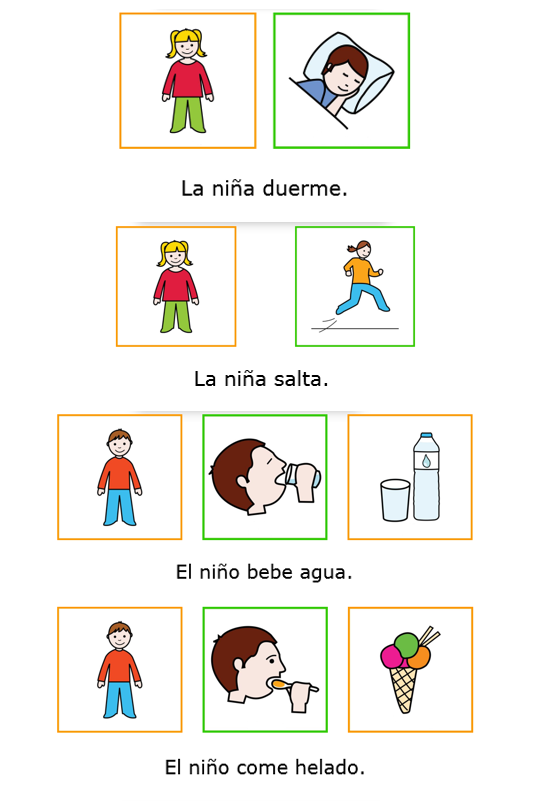
\includegraphics[width=7cm]{Imagenes/Apendice/ApendiceA/apendiceA1}
\end{figure}

\begin{figure}[h]
  \centering
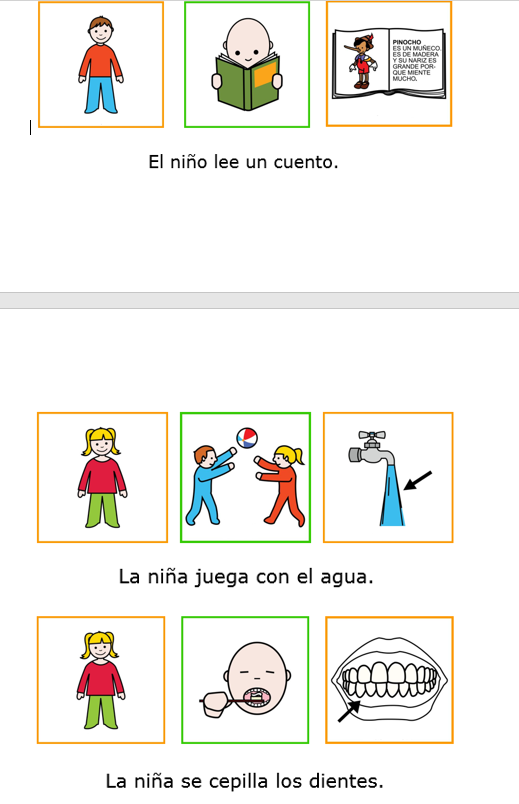
\includegraphics[width=5.9cm]{Imagenes/Apendice/ApendiceA/apendiceA2}
\end{figure}

\begin{figure}[h]
  \centering
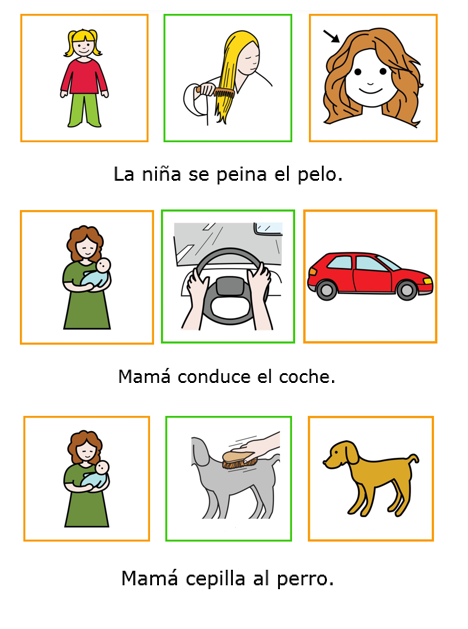
\includegraphics[width=5.9cm]{Imagenes/Apendice/ApendiceA/apendiceA3}
\end{figure}

\begin{figure}[h]
  \centering
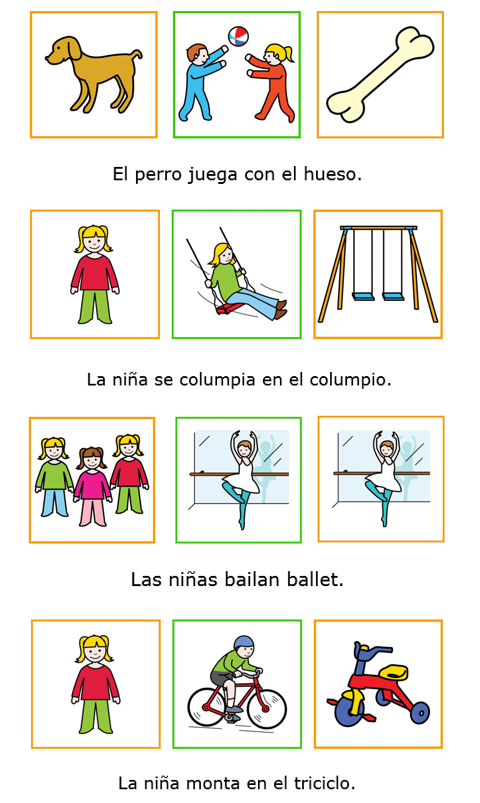
\includegraphics[width=5.9cm]{Imagenes/Apendice/ApendiceA/apendiceA4}
\end{figure}

\begin{figure}[h]
  \centering
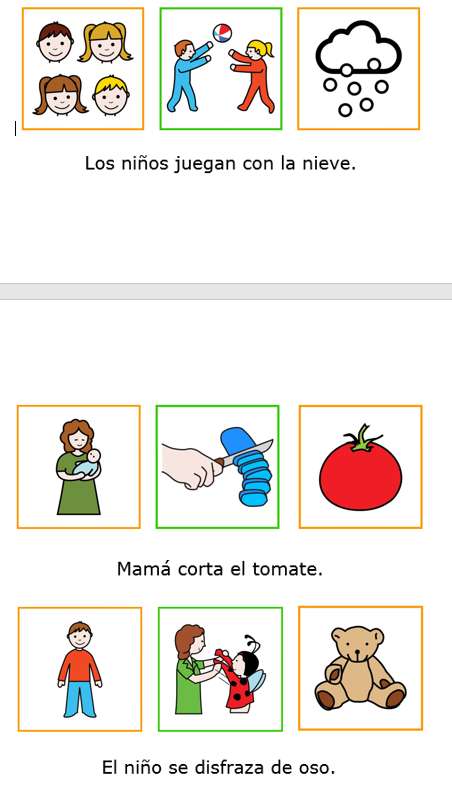
\includegraphics[width=5.9cm]{Imagenes/Apendice/ApendiceA/apendiceA5}
\end{figure}

\begin{figure}[h]
  \centering
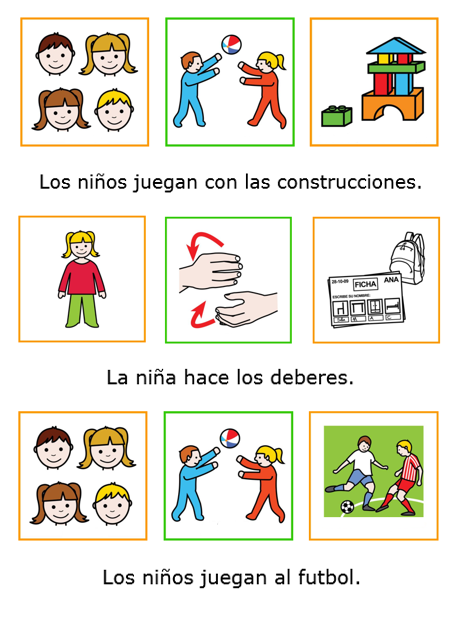
\includegraphics[width=5.9cm]{Imagenes/Apendice/ApendiceA/apendiceA6}
\end{figure}

\begin{figure}[h]
  \centering
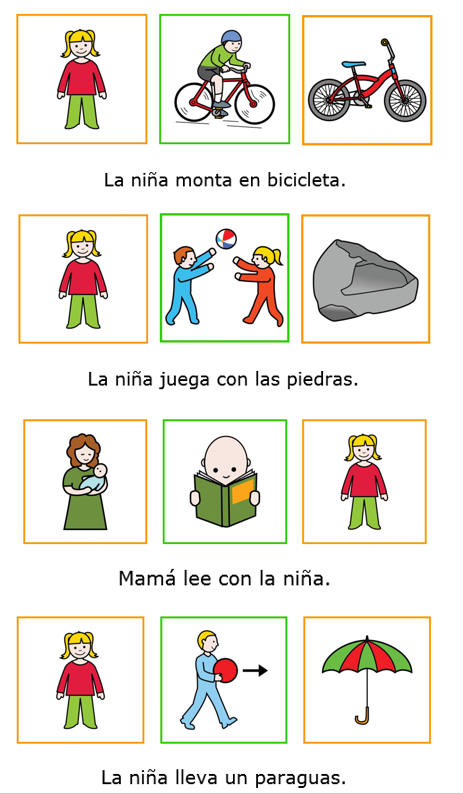
\includegraphics[width=5.9cm]{Imagenes/Apendice/ApendiceA/apendiceA7}
\end{figure}

\begin{figure}[h]
  \centering
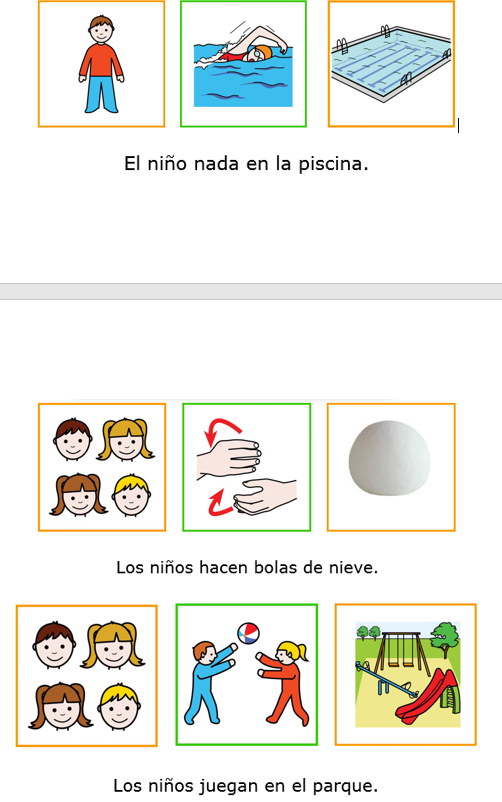
\includegraphics[width=7cm]{Imagenes/Apendice/ApendiceA/apendiceA8}
\end{figure}

\begin{figure}[h]
  \centering
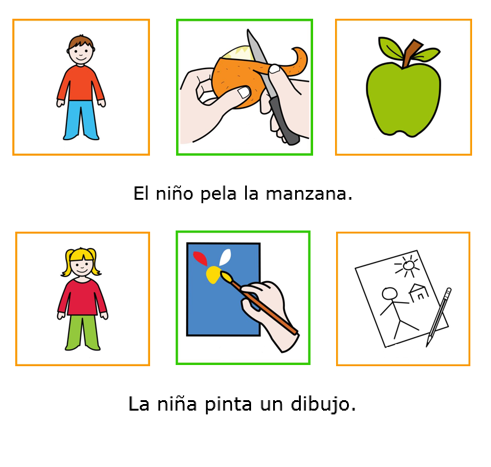
\includegraphics[width=7cm]{Imagenes/Apendice/ApendiceA/apendiceA9}
\end{figure}

\begin{figure}[h]
  \centering
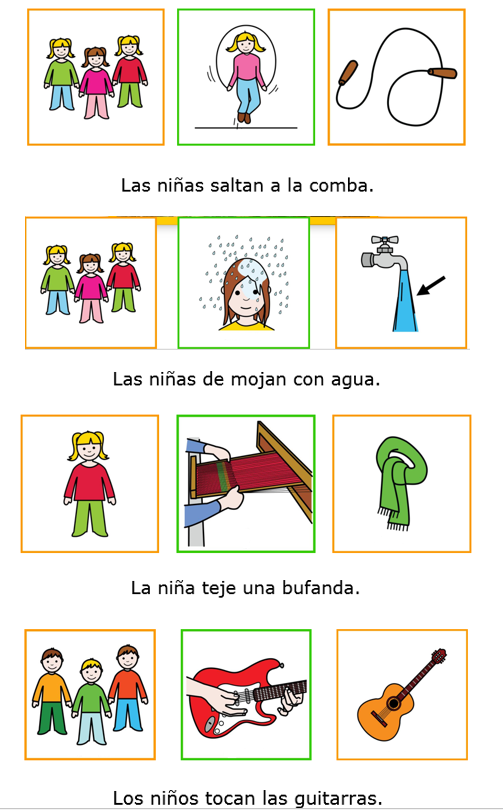
\includegraphics[width=7cm]{Imagenes/Apendice/ApendiceA/apendiceA10}
\end{figure}